\section{NPUcore内核代码结构及内核构建目标}
\subsection{NPUcore内核代码树}
下面是NPUcore的内核代码树:
\begin{figure}[htb]
	\centering
	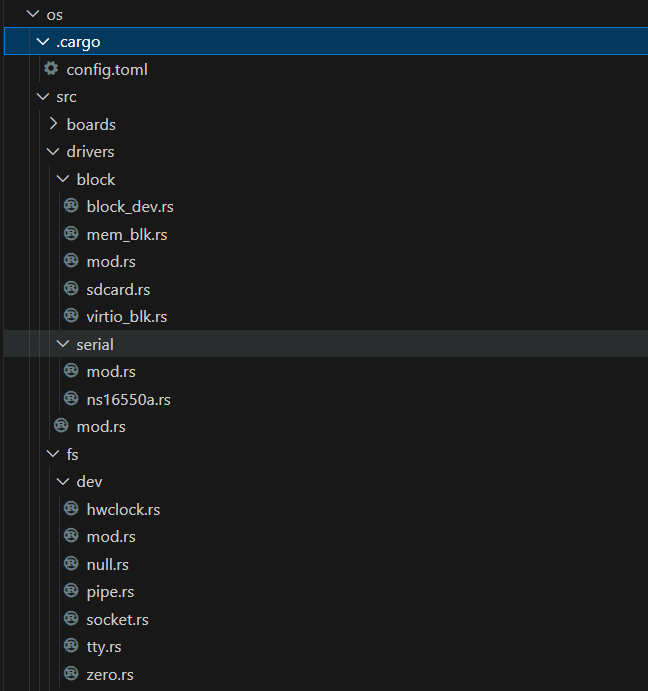
\includegraphics[width=\textwidth]{figures/02-03-内核代码树1.png}
	\caption{
		内核代码树1
	}
	\label{fig:内核代码树1}
\end{figure}

\begin{figure}[htb]
	\centering
	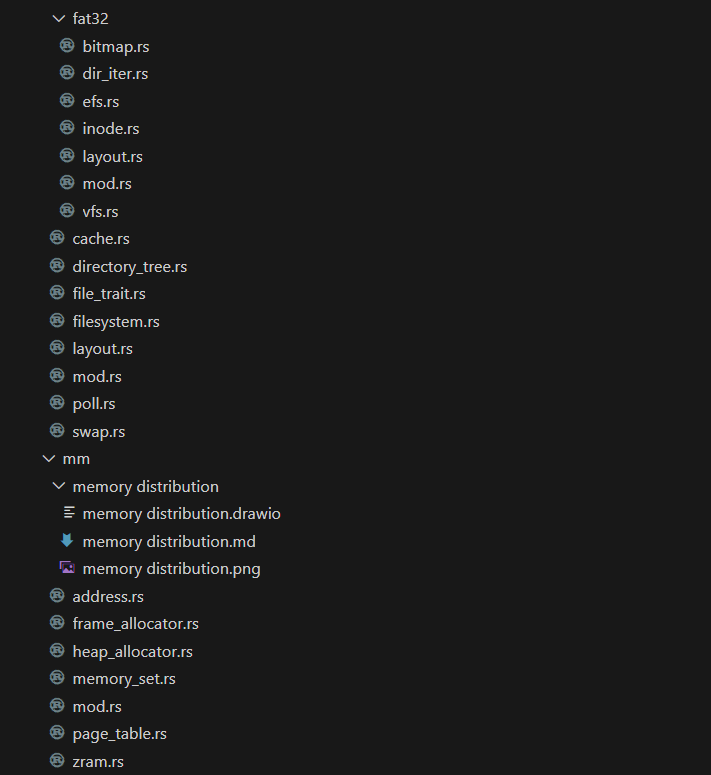
\includegraphics[width=\textwidth]{figures/02-03-内核代码树2.png}
	\caption{
		内核代码树2
	}
	\label{fig:内核代码树2}
\end{figure}

\begin{figure}[htb]
	\centering
	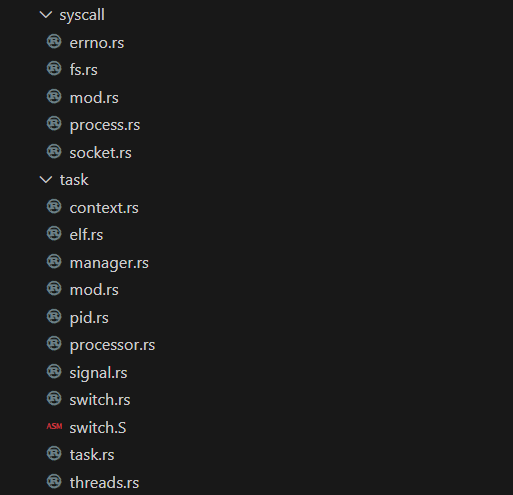
\includegraphics[width=\textwidth]{figures/02-03-内核代码树3.png}
	\caption{
		内核代码树3
	}
	\label{fig:内核代码树3}
\end{figure}

\begin{figure}[htb]
	\centering
	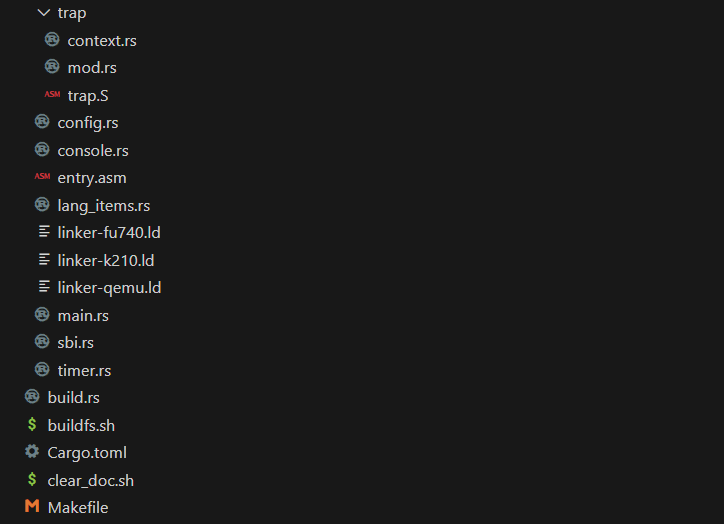
\includegraphics[width=\textwidth]{figures/02-03-内核代码树4.png}
	\caption{
		内核代码树4
	}
	\label{fig:内核代码树4}
\end{figure}


\subsection{NPUcore学习路线}
下面是我们为你准备的NPUcore的学习路线
\begin{figure}[htb]
	\centering
	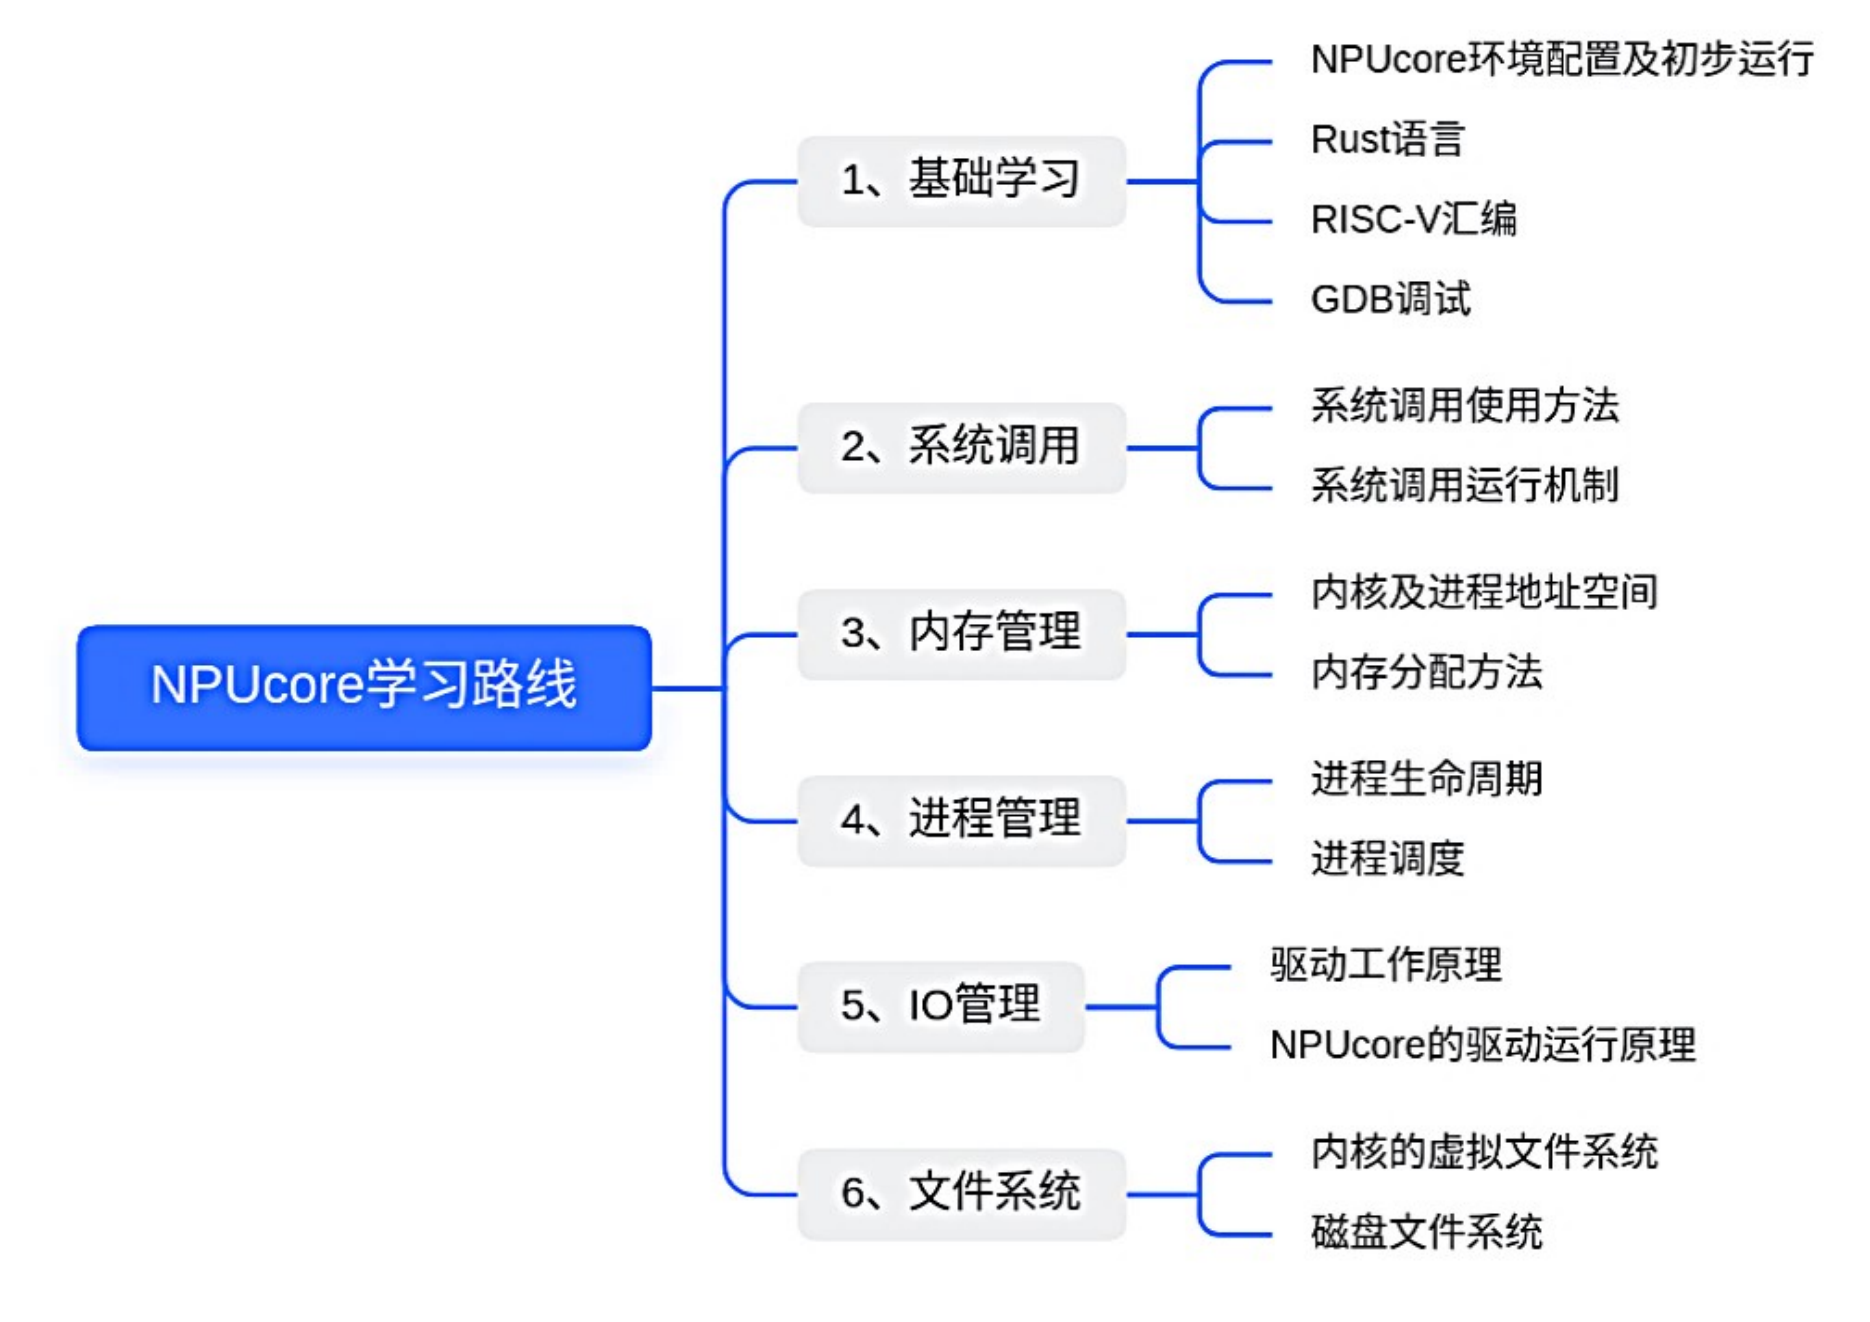
\includegraphics[width=\textwidth]{figures/02-03-NPUcore学习路线.png}
	\caption{
		NPUcore学习路线
	}
	\label{fig:NPUcore学习路线}
\end{figure}

希望你能渐渐的喜爱上操作系统~
